%!TEX root = ./Structure_rapport_final.tex

\subsection{Factorial Analysis of Mixed Data}

The first 5 FAMD components explained 80\% of the total variation (Table \ref{table:cont_abs}). The first principal component (PC1) (30.5\% of explained variance) is strongly correlated with shape of the body and of the head with traits such as \emph{body depth} (a = 11.7), \emph{lower jaw length} (a=11.5), \emph{oral gape axis} (a=11.1), orbital length (a = 8.35) and head length (a = 8.21), thus, mostly to feeding and locomotion (Table \ref{table:cont_abs}). Along this horizontal axis, all traits have increasing values toward the right, mouth orientation shifting upward (see Figure~\ref{fig:corr_circ_12} for details). Three groups of fish can be distinguished \ref{fig:famd12}. For low PC1 values, species have a low transversal shape (meaning that both \texttt{bd} and \texttt{bw} have similar values, consistent with an elongated body), short lower jaw, small oral gape surface and a terminal oral axis, such as \textit{A. risso}, \textit{S. boa} and \textit{S. beanii}. On the right of this axis, species display high body depth values suggesting a laterally compressed form and a superior-oriented oral axis, such as \textit{A. olfersii}. 

The second axis (21.6\% of explained variance) is correlated to feeding behavior, through food prospection with \emph{pectoral fin insertion} (a = 11.4), \emph{eye size} (a = 9), \emph{pectoral fin position} (a = 7.1) and food acquisition through \emph{gill raker type} (a = 17.8) and \emph{oral gape axis} (a = 12,3) (Table \ref{table:cont_abs}). This vertical axis separates the three species on the left, \textit{A. risso} and \textit{S. boa} display higher values of pectoral fin insertion, meaning that the fin is inserted further on the body than \textit{S. boa}, while the fin position on the body depth is lower. As \textit{S. beanii} does not have pectoral fin, same analysis has been run without traits referring to pectoral or pelvic fins to look and confirmed the discrimination between these species were highly dependant if these traits. Same results than Figure \ref{fig:famd12} were obtained.

The third axis (explaining 12.2\% of total variance) mainly carries traits linked to the foraging and swimming behavior, with strong influence of \emph{anus position} (a = 23.8), \emph{gill raker type} (a = 19.2), \emph{dorsal fin insertion} (a = 15.5) and \emph{pectoral fin position} (a = 14.2) (Table \ref{table:cont_abs}). On the left of this horizontal axis, species are characterized by a rather high pectoral fin insertion and close-to-head dorsal fin insertion and anus position (Figures \ref{fig:famd34} and \ref{fig:corr_circ_34}).
Finally, the fourth axis (explaining 7.9\% of variance) is mainly related to feeding and habitat traits, with \emph{pyloric caeca} (a = 31.6), \emph{operculum volume} (a = 17) and \emph{presence of photophores} (a = 10.9) (Table \ref{table:cont_abs}). Because \textit{X. copei} is the only species having pyloric caeca, this variable clearly separates that species from the other, on the PC4 axis. The remaining PC scores (20\% of variance) are mainly linked to food acquisition. Overall, FAMD analysis detects similarities between species niches', with ellipses overlapping. Conversely, some species are well segregated along these first four axis, suggesting the existence of several functional groups within studied community. 

Because PC1 and PC2 have most of the weight in the functional analysis, it suggests that the traits they carry are the most relevant to segregate species. In particular, \emph{lower jaw length}, \emph{body depth}, \emph{pectoral fin insertion} and \emph{eye size} are the quantitative traits that are the most distinct among species and helps to distinguish them. As for qualitative variables, it seems that \emph{oral gape axis} and \emph{gill raker type} are the one which separates the most species. This makes sense considering they have the most modalities, allowing a more precise description than binaries \emph{presence of photophores} and \emph{pyloric caeca} scores. 


% Table of contributions of variables for 5 first axis
\begin{table}[!htbp]
\centering
\caption[Correlations values of fifth first principal component and functional traits]{Correlation between 5 first PC's and functional traits. In bold, correlations higher than threshold (4.8).}
\label{table:cont_abs}
\begin{adjustbox}{max width=1.1\textwidth,center}
\begin{tabular}{>{\bfseries}crrrrrr}
  \hline
 Function & Trait & PC1 (30.5\%) & PC2 (21.6\%) & PC3 (12.2\%) & PC4 (7.9\%) & PC5 (7.8\%) \\ 
  \hline
  \multirow{13}{*}{Feeding} &Oral gape axis & \textbf{11.07} & \textbf{12.28} & 3.32 & 3.27 & \textbf{7.13} \\ 
  &Eye size & 1.29 & \textbf{9.01} & 3.52 & 4.08 & 1.40 \\ 
  &Orbital length & \textbf{8.35} & 2.38 & 0.00 & 2.24 & 4.54 \\ 
  &Oral gape surface & \textbf{7.78} & 3.06 & 2.93 & 0.10 & 2.78 \\ 
  &Oral gape shape & 0.18 & 3.10 & 0.05 & \textbf{9.49} & \textbf{10.41} \\ 
  &Oral gape position & 0.42 & 1.21 & 1.99 & \textbf{9.16} & 3.94 \\ 
  &Lower jaw length & \textbf{11.52} & 0.00 & 0.04 & 1.97 & 2.44 \\ 
  &Gill raker type & 4.38 & \textbf{17.80} & \textbf{19.23} & 0.32 & 3.42 \\ 
  &Gill outflow & \textbf{5.47} & 0.82 & 0.02 & 2.22 & \textbf{22.48} \\ 
  &Head length & \textbf{8.21} & 3.10 & 2.50 & 0.78 & 4.50 \\ 
  &Pyloric caeca & 0.23 & 0.48 & 0.04 & \textbf{31.62} & \textbf{5.81} \\ 
  &Anus position & 0.00 & \textbf{5.28} & \textbf{23.81} & 0.07 & 0.77 \\ 
   \hline
   \multirow{6}{*}{Locomotion} & Body depth & \textbf{11.68} & 0.93 & 1.41 & 0.64 & 1.92 \\ 
  &Pectoral fin position & 1.72 & \textbf{7.15} & \textbf{14.22} & 0.37 & 0.32 \\ 
  &Pectoral fin insertion & \textbf{4.95} & \textbf{11.39} & 0.05 & 0.12 & 0.74 \\ 
  &Transversal shape & \textbf{5.96} & 4.33 & 5.45 & 1.70 & 2.10 \\ 
  &Caudal throttle width & 3.72 & \textbf{5.01} & 0.28 & 1.60 & \textbf{16.30} \\ 
  &Dorsal fin insertion & 2.58 & 4.78 & \textbf{15.52} & 0.00 & 1.33 \\ 
  \hline
  \multirow{2}{*}{Habitat} &Eye position & 0.19 & \textbf{5.41} & 0.78 & 2.34 & 1.40 \\ 
  &Presence photophores & \textbf{7.79} & 2.45 & 3.23 & \textbf{10.89} & 0.59 \\
  &Operculum volume & 2.52 & 0.03 & 1.61 & \textbf{17.02} & \textbf{5.68} \\ 
   \hline
\end{tabular}
\end{adjustbox}
\end{table}

% Plot of FAMD axis 1 and 2
\newgeometry{left=1cm,right=1cm,bottom=1.5cm,top=1cm}
\begin{figure} [!htbp]
	\begin{center}
		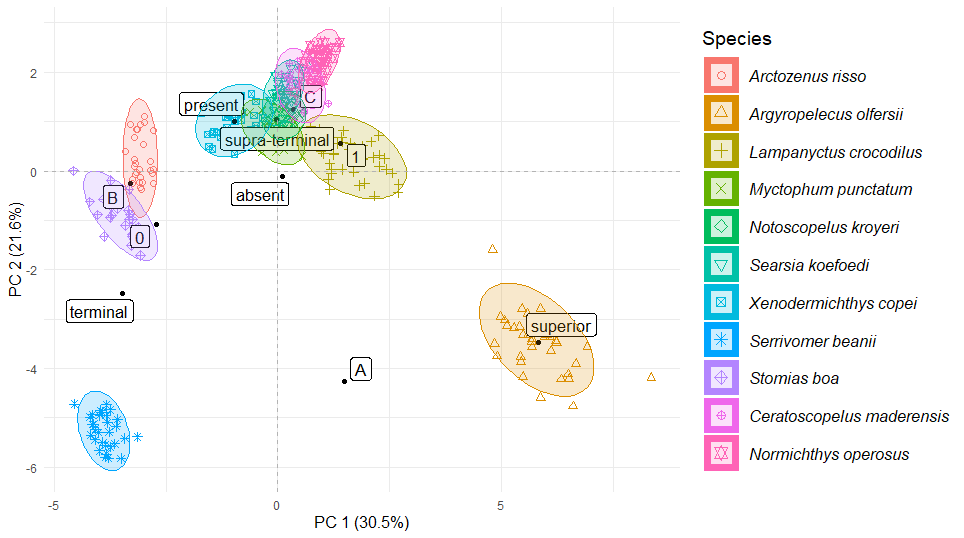
\includegraphics[width=\textwidth]{FAMD12.png}  
	\end{center}
	\caption[FAMD results for first and second axis]{FAMD results for PC 1 and 2. Framed variables are scores of categorical variables.}
	\label{fig:famd12}
\end{figure}

% Plot of FAMD axis 3 and 4
\begin{figure} [!htbp]
	\begin{center}
		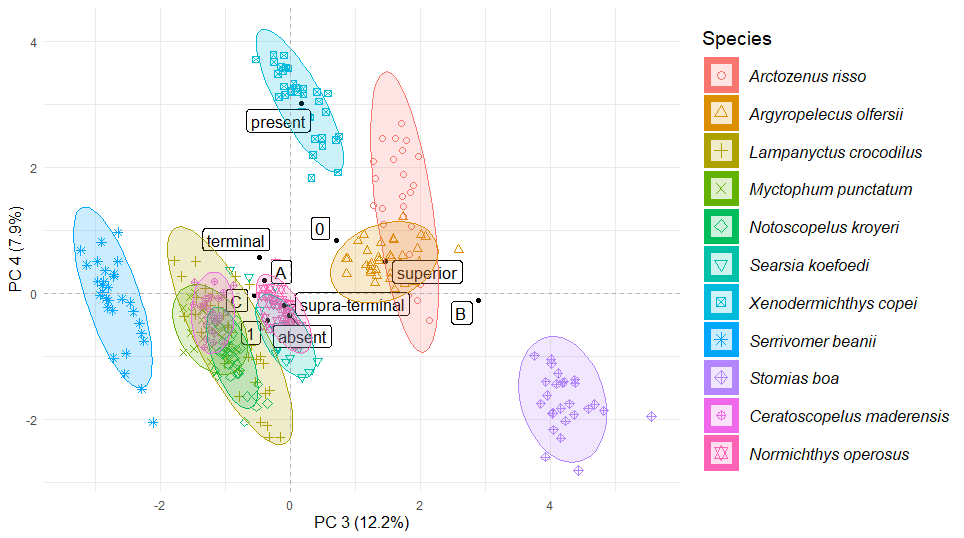
\includegraphics[width=\textwidth]{FAMD34.png}
	\end{center}
	\caption[FAMD results for third and fourth axis]{FAMD results for PC 3 and 4. Framed variables are scores of categorical variables.}
	\label{fig:famd34}
\end{figure}
\restoregeometry


\subsection{Functional niche surface and overlap}
Overall, several species' ellipses overlaps on these first four principal components (Figures \ref{fig:famd12} and \ref{fig:famd34}). For these species, the aim is now to measure the intensity of these overlaps. On the first and second principal components, all 4 Myctophidae and 2 Platytroctidae species, plus \textit{X. copei} are more or less overlapping, not displaying much differences along PC1 nor PC2 (Figure \ref{fig:famd12}). \textit{A. risso} and \textit{S. boa} seems to slightly overlap each other niches, which are mainly separated along PC2 (Figure \ref{fig:famd12}). \textit{S. beanii} and \textit{A. olfersii} are the only two species not showing any overlap. 
Being opposed in the first two dimensions (Figure \ref{fig:famd12}), \textit{A.risso} and \textit{A. olfersii} nonetheless seem to share some of their foraging strategiy, with their niche partly overlapping (Figure \ref{fig:famd34}). As for overlapping species of Figure \ref{fig:famd12}, segregation among families is observed (Figure \ref{fig:famd34}). Firstly, \textit{X. copei}'s niche is now fully segregated from other species. Both Platytroctidae are gathered and separated from \textit{C. maderensis}, \textit{M. punctatum} and \textit{N. kroyeri}. The last Myctophidae species, \textit{L. crocodilus}, which have the widest niche among these species, is not fully segregated and show some overlaps with \textit{S. koefoedi}.

The niche surface estimation showed that \textit{N. kroyeri} had the narrowest niche among the studied community, followed by \textit{N. operosus} and \textit{S. koeofedi} (Table \ref{table:sp_surface}). Then, \textit{C. maderensis}, \textit{A. risso}, \textit{S. beanii} and \textit{M. punctatum}, \textit{S. boa} and \textit{X. copei} all have niches almost two to three times wider than \textit{N. kroyeri}'s. Finally, comparing to \textit{N. kroyeri}'s niche, \textit{L. crocodilus}'s is four time wider, while \textit{A. olfersii}'s is more than seven time wider. In fact, all Myctophidae (except \textit{L. crocodilus}) and Platytroctidae have rather small niches and are the one overlapping in Figure \ref{fig:famd12}.

Bootstrapped niche surface estimation did not show any difference in the surface of estimated niche through sample size \textit{n}. Hence, surface of niches seems to be more influenced by the trait variability of the sampled individuals rather than the number of individuals itself. Yet, estimated niche surface value are tightly converging for \textit{n} = 30. 

% Niche standardardised surfaces
\begin{table}[!htbp]
\centering
\caption[Standardized surface of functional niches]{Standardized surface of functional niches.}
\label{table:sp_surface}
\begin{adjustbox}{max width=1.1\textwidth,center}
\begin{tabular}{lr}
  \hline
Species & Relative surface \\ 
  \hline
Argyropelecus olfersii & 7.4 \\ 
  Lampanyctus crocodilus & 4.0 \\ 
  Xenodermichthys copei & 2.6 \\ 
  Stomias boa & 2.5 \\ 
  Myctophum punctatum & 2.1 \\ 
  Serrivomer beanii & 1.9 \\ 
  Arctozenus risso & 1.8 \\ 
  Ceratoscopelus maderensis & 1.7 \\ 
  Searsia koefoedi & 1.3 \\ 
  Normichthys operosus & 1.2 \\ 
  Notoscopelus kroyeri & 1.0 \\ 
   \hline
\end{tabular}
\end{adjustbox}
\end{table}

Niche overlap analysis confirms that 9 species show overlapping niches with at least one other species (Figure \ref{fig:famd12}) and that smallest niches overlaps each other the most (Table \ref{table:ell_ovlp}). The maximum  overlap is found between \textit{M. punctatum} and \textit{N. kroyeri}, as almost 69\% of the latter's niche is covered by the first. In total, these two species share 22\% of their niches. \textit{S. koefoedi} is sharing more than 28\% of its niche with both \textit{C. maderensis} and \textit{N. kroyeri}, which are the two highest total overlap values here (Table \ref{table:ell_ovlp}). Overall, \textit{N. kroyeri}'s niche is fully overlapped by six other species. \textit{C. maderensis}, \textit{S. koefoedi} and \textit{M. punctatum} are overlapping five other species. Finally, \textit{L. crocodilus}, \textit{X. copei} and \textit{N. operosus} are involved in overlap with three other species, and \textit{A. risso} and \textit{S. boa} are only overlapping each other (Table \ref{table:ell_ovlp}). Finally, \textit{N. kroyeri} and \textit{N. operosus} show minimum total overlap value of 0.2\%, which might no be significative and mostly due to some individuals of the latter in \textit{N. kroyeri}'s ellipse (Figure \ref{fig:famd12}). 

\begin{table}[!htbp]
\centering
\caption[Overlap of species' ellipses]{Species' ellipses overlap. All the others comparisons that are not present in this table did not present any overlap.}
\label{table:ell_ovlp}
\begin{adjustbox}{max width=1.1\textwidth,center}
\begin{tabular}{llrrr}
  \hline
Species1 & Species2 & Total overlap (\%) &  Overlap of Species 2 over Species 1 (\%) & Overlap of Species 1 over Species 2 (\%) \\ 
  \hline
Searsia koefoedi & Ceratoscopelus maderensis & 28.20 & 65.40 & 49.60 \\ 
  Notoscopelus kroyeri & Searsia koefoedi & 28.10 & 65.40 & 49.20 \\ 
  Myctophum punctatum & Notoscopelus kroyeri & 22.00 & 32.30 & 68.70 \\ 
  Myctophum punctatum & Xenodermichthys copei & 20.20 & 44.90 & 36.60 \\ 
  Ceratoscopelus maderensis & Normichthys operosus & 19.00 & 31.80 & 47.10 \\ 
  Notoscopelus kroyeri & Ceratoscopelus maderensis & 15.10 & 41.60 & 23.70 \\ 
  Myctophum punctatum & Searsia koefoedi & 12.50 & 20.30 & 32.40 \\ 
  Searsia koefoedi & Normichthys operosus & 7.90 & 15.00 & 16.90 \\ 
  Notoscopelus kroyeri & Xenodermichthys copei & 6.40 & 22.90 & 8.80 \\ 
  Searsia koefoedi & Xenodermichthys copei & 5.90 & 17.50 & 8.90 \\ 
  Lampanyctus crocodilus & Myctophum punctatum & 4.20 & 6.50 & 12.20 \\ 
  Arctozenus risso & Stomias boa & 3.90 & 9.40 & 6.60 \\ 
  Myctophum punctatum & Ceratoscopelus maderensis & 3.20 & 5.80 & 7.00 \\ 
  Lampanyctus crocodilus & Ceratoscopelus maderensis & 1.70 & 2.50 & 5.70 \\ 
  Lampanyctus crocodilus & Notoscopelus kroyeri & 1.00 & 1.20 & 4.80 \\ 
  Notoscopelus kroyeri & Normichthys operosus & 0.20 & 0.50 & 0.40 \\ 
   \hline
\end{tabular}
\end{adjustbox}
\end{table}

Niche's distinctiveness informs on functional diversity of species within a community, increasing values meaning that, locally, species display rarer functions. Here, Myctophidae and Playtroctidae families are all equally functionally distinct from one another (Table \ref{table:nich_diss}). Even if the values are rather close, \textit{S. koefoedi} and \textit{M. punctatum} seems to be the most alike species. Conversely, \textit{A. olfersii}, \textit{S. beanii} and \textit{S. boa} tend to have more distinct niches, which are consistent with previous results (Figure \ref{fig:famd12}). Here, species with the most atypical morphological feature are the more distinct in terms of niche. 

\begin{table}[!htbp]
\centering
\caption[Dissimilarities values of species' niches]{Niche dissimilarity of studied species}
\label{table:nich_diss}
\begin{adjustbox}{max width=1.1\textwidth,center}
\begin{tabular}{lr}
  \hline
Species & Distinctiveness value \\ 
  \hline
Argyropelecus olfersii & 0.54 \\ 
  Serrivomer beanii & 0.51 \\ 
  Stomias boa & 0.46 \\ 
  Arctozenus risso & 0.40 \\ 
  Lampanyctus crocodilus & 0.37 \\ 
  Xenodermichthys copei & 0.37 \\ 
  Ceratoscopelus maderensis & 0.31 \\ 
  Normichthys operosus & 0.31 \\ 
  Notoscopelus kroyeri & 0.30 \\ 
  Searsia koefoedi & 0.29 \\ 
  Myctophum punctatum & 0.29 \\  
   \hline
\end{tabular}
\end{adjustbox}
\end{table}


\subsection{Kernel density estimation}
Kernel density estimation helps to understand which are the traits that have the same distributions for species. Looking at these distributions for overlapping species gives information on traits, and thus, functions similarities among species. The estimation of kernel density for the 7 overlapping species shows that these species are overlapping for 7 of the 17 computed traits (Figure \ref{fig:dpo}; Table \ref{table:kern_over_val}). The overlap is maximum for \emph{oral gape position} (trait n°5) with an overlap value of 0.34. This means that, along this functional trait, these 6 species share nearly 34\% of the trait density distribution. For this trait, most of the distributions are centered around a range of values of [0.5-0.8], yet \textit{L. crocodilus} display a pretty wide distribution, despite being the most sampled species (Table \ref{table:spcount}). This same observation can be done for this particular species for \emph{body depth} (trait n°11) and \emph{pectoral fin insertion} (trait n°13). Species also share nearly 25\% and 29\% of their density when looking at \emph{body depth} (trait n°11) and \emph{eye position} (trait n°17), respectively. Finally, \emph{lower jaw length} (trait n°6) and \emph{pectoral fin position} (trait n°12) values also seem to be common to those species, with 16\% and 19\% of density shared, respectively. To a lesser extent, species share nearly 12\% of the \emph{eye size} values (trait n°2).

Furthermore, we can notice that \emph{oral gape surface} (trait n°3), \emph{operculum volume} (trait n°8) and \emph{pectoral fin insertion} (trait n°13) display bimodal distributions (Figure \ref{fig:dpo}. For these traits, \textit{L. crocodilus}, \textit{N. operosus} and \textit{S. koefoedi} constitutes one mode, and the resting species the other. Conversely, \emph{eye size} (trait n°1) shows multimodal distribution, with nearly every species having its proper mode.

For most traits, \textit{N. kroyeri} (green) and \textit{M. punctatum} (blue) have very similar distributions (\ref{fig:dpo}). When looking at these two species only, analysis show that they are overlapping for every 17 traits, with particularly high values for \emph{eye size} (o = 0.915), \emph{operculum volume} (o = 0.901), \emph{gill outflow} (o = 0.882), \emph{pectoral fin insertion} (o = 0.828) and \emph{caudal throttle width} (o = 0.782), with the mean overlap of the 17 traits being $\bar{o}$ = 0.561.


\begin{table}[!htbp]
\centering
\caption[Kernel density overlap values for the 17 traits]{Kernel density overlap values for the 17 computed traits for the seven overlapping species. Values in bold are significant (p < 0.01) and shown in Figure \ref{fig:dpo}.}
\label{table:kern_over_val}
\begin{adjustbox}{max width=1.1\textwidth,center}
\begin{tabular}{lcr}
  \hline
Trait code & Functional trait & Total overlap (o) \\ 
  \hline
1 & Eye size & 0.00 \\ 
  2 & Orbital length & \textbf{0.12} \\ 
  3 & Oral gape surface & 0.00 \\ 
  4 & Oral gape shape &0.00 \\ 
  5 & Oral gape position & \textbf{0.34} \\ 
  6 & Lower jaw length & \textbf{0.16} \\ 
  7 & Gill outflow & 0.00 \\ 
  8 & Operculum volume & 0.00 \\ 
  9 & Head length & 0.00 \\ 
  10 & Anus position & 0.00 \\ 
  11 & Body depth & \textbf{0.25} \\ 
  12 & Pectoral fin position & \textbf{0.20} \\ 
  13 & Pectoral fin insertion & \textbf{0.01} \\ 
  14 & Transversal shape & 0.00 \\ 
  15 & Caudal throttle width & 0.00 \\ 
  16 & Dorsal fin insertion & 0.00 \\ 
  17 & Eye position & \textbf{0.29} \\ 
   \hline
\end{tabular}
\end{adjustbox}
\end{table} 

\begin{figure} [!htbp]
	\begin{center}
		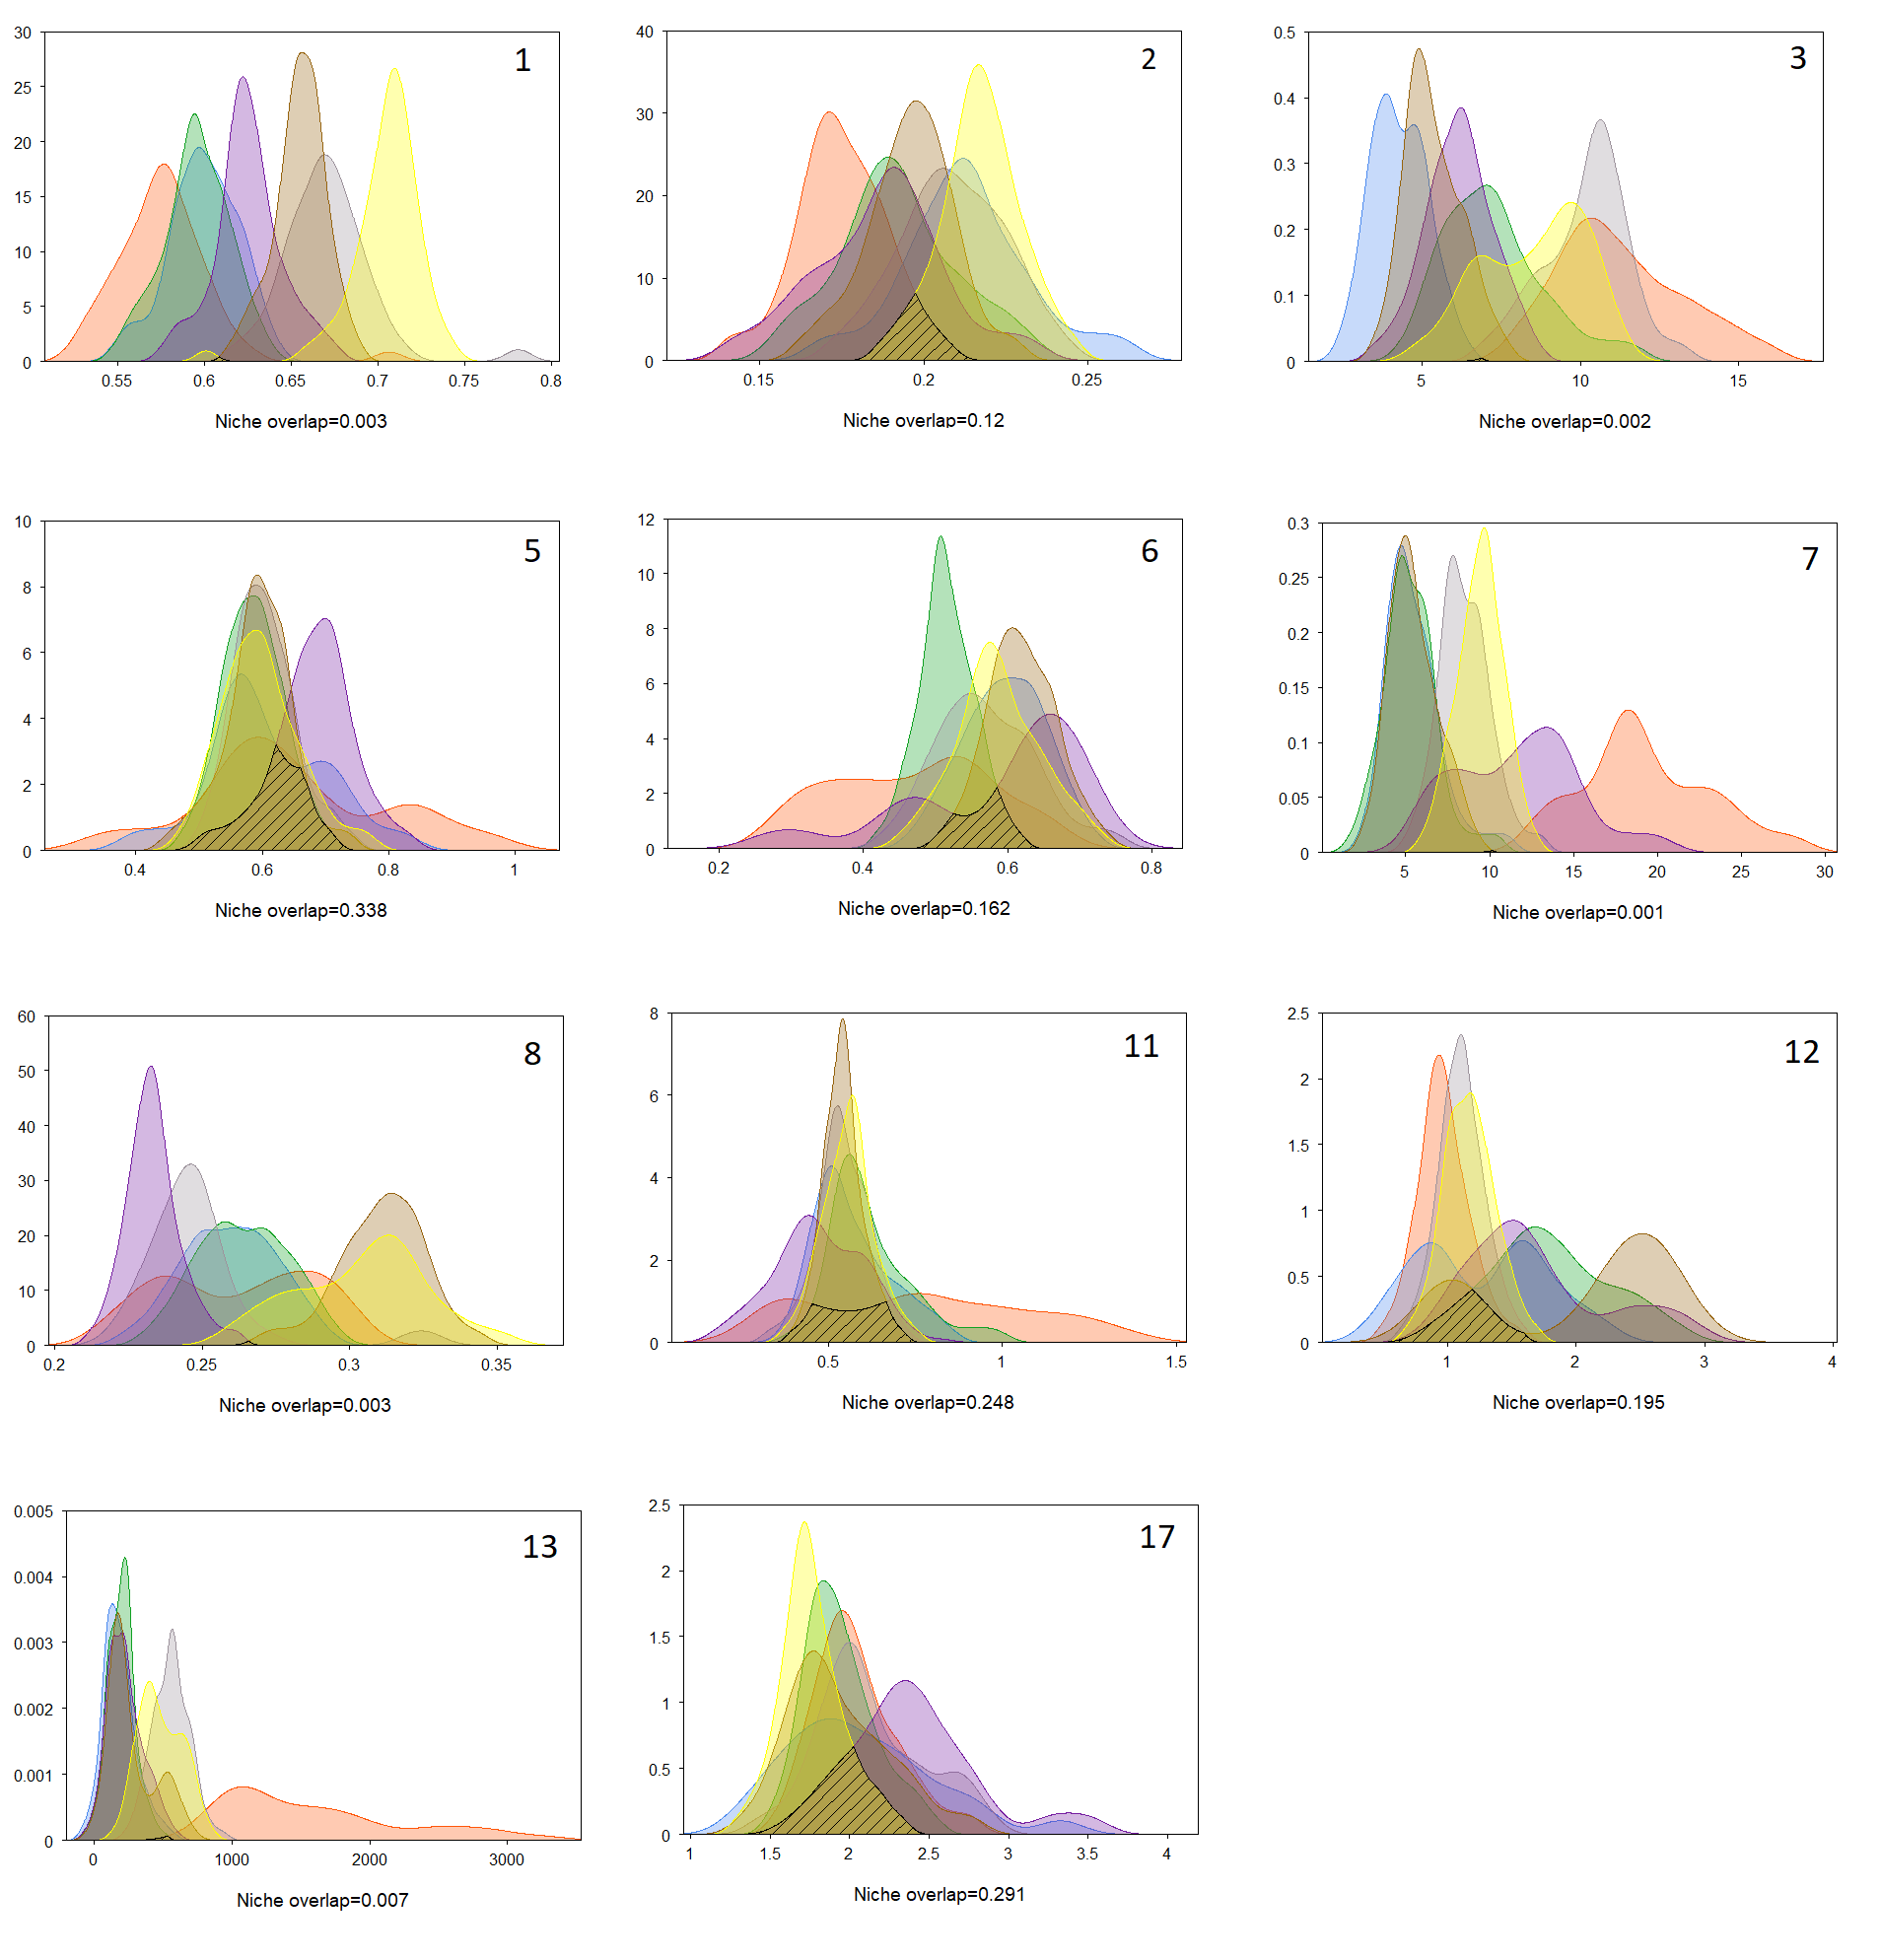
\includegraphics[width=\textwidth]{Density_plot.png}
	\end{center}
	\caption[Kernel density distribution of overlapping species]{Kernel density overlap for 11 functional traits and the overlaping species. Colors correspond to following species: orange - \textit{L. crocodilus}; brown - \textit{C. maderensis}; yellow - \textit{N. operosus}; purple - \textit{X. copei}; green - \textit{N. kroyeri}; blue - \textit{M. punctatum}; grey - \textit{S. koefoedi}. Overlap is represented by shaded lines. Here, are displayed every traits that showed non-null overlap.}
	\label{fig:dpo}
\end{figure}